\documentclass{standalone}
\usepackage{tikz}
\begin{document}
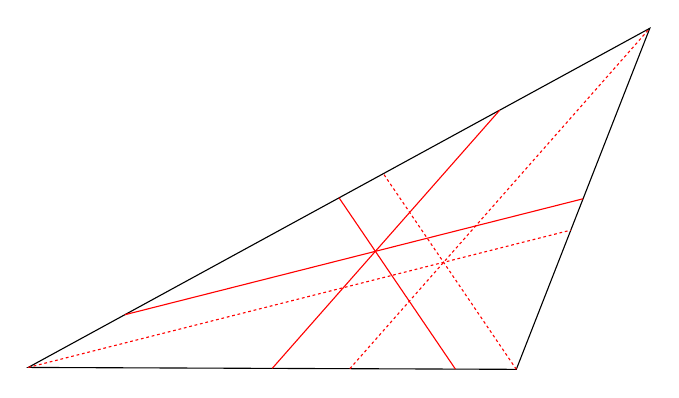
\begin{tikzpicture}[x=1pt,y=1pt]
\draw (45.25,-148.11) -- (221.62,-148.80) -- (269.86,-25.55) -- cycle;
\draw[red] (80.15,-129.07) -- (245.73,-87.17);
\draw[red] (199.61,-148.71) -- (157.56,-86.82);
\draw[red] (133.43,-148.44) -- (215.65,-55.12);
\draw[red, dash pattern=on 1pt] (221.62,-148.79) -- (173.56,-78.08);
\draw[red, dash pattern=on 1pt] (45.25,-148.11) -- (241.29,-98.50);
\draw[red, dash pattern=on 1pt] (161.48,-148.56) -- (269.86,-25.54);
\end{tikzpicture}
\end{document}
